\section[Hermitesche VR und Hauptachsentrafo]{Hermitesche Vektorräume, Selbstadjungierte Endomorphismen, Hauptachsentransformation}
\Einleitung{Heute werden wir uns genauer mit einer speziellen Klasse von Basen\footnote{mit paarweise orthogonalen Basisvektoren der Länge 1} und einem einprägsamen Verfahren zur Findung derselben beschäftigen und zudem den Begriff des euklidischen Skalarprodukts, den wir von reellen Vektorräumen kennen, auf komplexe Vektorräume erweitern.\\
Hinter diesem sog. hermiteschen Skalarprodukt steht anstelle der Bilinearform die hermitesche Form, die der Bilinearform sehr ähnlich ist.\\
Danach lernen wir verschiedene wichtige Spezialfälle von Endomorphismen\footnote{Ein allerallerletztes Mal: Lineare Abbildungen eines Vektorraums in sich selbst.} auf euklidischen/\\hermiteschen Vektorräumen kennen. Diese haben besondere Eigenschaften:\\
Für orthogonale (in reellen VR) bzw. unitäre (in komplexen VR) Endomorphismen stehen Eigenvektoren senkrecht aufeinander.\\
Selbstadjungierte Endomorphismen treiben das Ganze noch weiter und wir sehen, dass wir diese mit dem Skalarprodukt identifizieren\footnote{genauer: es herrscht Isomorphie} können.\\
Das alles schließen wir mit der Erkenntnis ab, dass sich Bilinearformen bzw. hermitesche Formen bezüglich einer Basis des Vektorraumes mithilfe einer darstellenden Matrix in Diagonalgestalt darstellen lassen, welche nur $-1,1$ und $0$ als Einträge hat.\\
Für symmetrische Bilinearformen wird dieser Prozess auch Hauptachsentransformation genannt.}

\subsection{Orthonormale Basen: Ausgezeichneter geht kaum mehr}
\begin{Def}
{Orthonormalbasis}
Wir nennen eine Basis $B$ eines euklidischen\footnote{es handelt sich also um einen reellen Vektorraum, auf dem ein Skalarprodukt definiert ist.} Vektorraumes \red{Orthonormalbasis}, wenn:
\begin{itemize}
	\item $\Norm{\bvec_i}=1\,\forall \bvec_i\in B$, \blue{die Basisvektoren sind \red{Einheitsvektoren} der Länge 1.}
	\item $\BiFo{\bvec_i,\bvec_j}=0\iff \bvec_i\perp \bvec_j\forall i\neq j,\, \bvec_i,\bvec_j\in B$, \blue{Basisvektoren sind paarweise orthogonal}.
\end{itemize}
Zusammengefasst gilt also $\boxed{\BiFo{\bvec_i,\bvec_j}=\delta_{ij}}$ für orthonormale Basisvektoren.
\end{Def}

\begin{Beispiel}
{Kommentar zu Einheitsvektoren}
Wir können aus jedem Vektor $\vvec\neq0$ einen Einheitsvektor konstruieren, indem wir durch dessen Länge $\Norm{\vvec}$ teilen.\\
Als Beispiel betrachten wir $\vvec=\MatrixInline{3\\6\\2}$ bzgl. des kanonischen Skalarproduktes. Wir haben
\begin{equation*}
	\Norm{\vvec}=\sqrt{\BiFo{\vvec,\vvec}}=\sqrt{9+36+4}=7.
\end{equation*}
Der normierte Vektor ist also $\hat{\evec}_\vvec=\frac{1}{7}\MatrixInline{3\\6\\2}$.
\end{Beispiel}

\begin{Satz}
{Satz}{Zur linearen Unabhängigkeit}
Für eine Familie von Vektoren $(\vvec_i)_{i\in J}$ mit $\vvec_i\in V\setminus\MengeDirekt{0}$ aus einem euklidischen Vektorraum gilt:
\begin{equation*}
	\BiFo{\vvec_i,\vvec_j}=0\quad\forall i\neq j\implies (\vvec_i)_{i\in J} \tx{ ist linear unabhängig}.
\end{equation*}
Wir so oft gilt die andere Richtung nicht, Achtung!
\end{Satz}
\begin{Satz}{Satz}{Von Gram-Schmidt}
Jeder endlichdimensionale euklidische Vektorraum besitzt eine Orthonormalbasis.\\
\blue{Diese ist nicht eindeutig.}
\end{Satz}
Dieser Satz gibt uns die Gewissheit, dass wir mit dem folgenden Verfahren aus einer gegebenen Basis stets eine Orthonormalbasis konstruieren können.\\
Das Normieren geht einfach - aber wie bekommen wir es hin, dass alle resultierenden Basisvektoren paarweise orthogonal sind?\\
Als Motivation konzentrieren wir uns auf die geometrische Bedeutung von Operationen mit Vektoren.
\begin{Wiederholung}
{Geometrische Bedeutung des Skalarproduktes}
\begin{wrapfigure}{r}[0pt]{.25\textwidth}
 \vspace{-15pt}
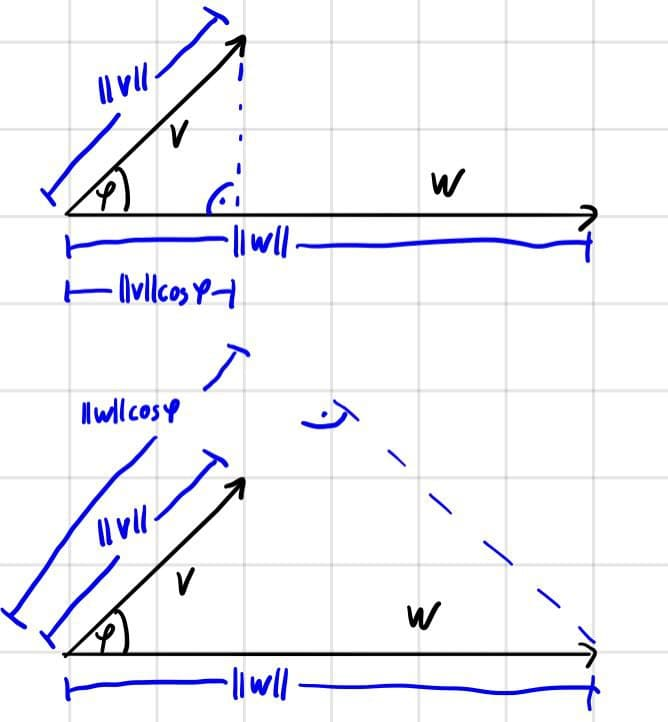
\includegraphics[width=.25\textwidth]{Dateien/04/04Skalarprodukt.jpg}
 \vspace{-15pt}
\end{wrapfigure}
Wir hatten den Winkel zweier Vektoren $\vvec,\wvec\in V\setminus\MengeDirekt{\Vec{0}}$\footnote{wobei $V$ ein euklidischer VR, d.h. ein VR mit einem Skalarprodukt ist} als
\begin{equation*}
    \angle(\vvec,\wvec):=\arccos\frac{\BiFo{\vvec,\wvec}}{\Norm{\vvec}\cdot\Norm{\wvec}}\in[0,\pi]
\end{equation*}
definiert, was anders aufgeschrieben $\BiFo{\vvec,\wvec}=\Norm{\vvec}\cdot\Norm{\wvec}\cos\varphi$ ist.\\
\blue{Das Skalarprodukt multipliziert also die Längen der Vektoren und berücksichtigt dabei den eingeschlossenen Winkel.\\
Tatsächlich ist es die Projektion der Vektoren $\vvec$ und $\wvec$ aufeinander, die multipliziert wird (siehe Skizze).}
\end{Wiederholung}
\blue{Mit dieser Erklärung wird vielleicht auch klar, weshalb $\BiFo{\vvec,\wvec}=0\iff \vvec\perp \wvec$ und\\
$\Abs{\BiFo{\vvec,\wvec}}=\Norm{\vvec}\cdot\Norm{\wvec}\iff \vvec,\wvec$ linear abhängig.}
\newpage
Bei dem gleich folgenden Verfahren ist es nützlich, im Kopf zu haben, was die verschiedenen Operationen von Vektoren anschaulich im $\mathbb{R}^2$ bedeuten:
\begin{Wiederholung}
{Addition und Subtraktion von Vektoren im $\mathbb{R}^2$}
\begin{wrapfigure}{r}[0pt]{.15\textwidth}
 \vspace{-15pt}
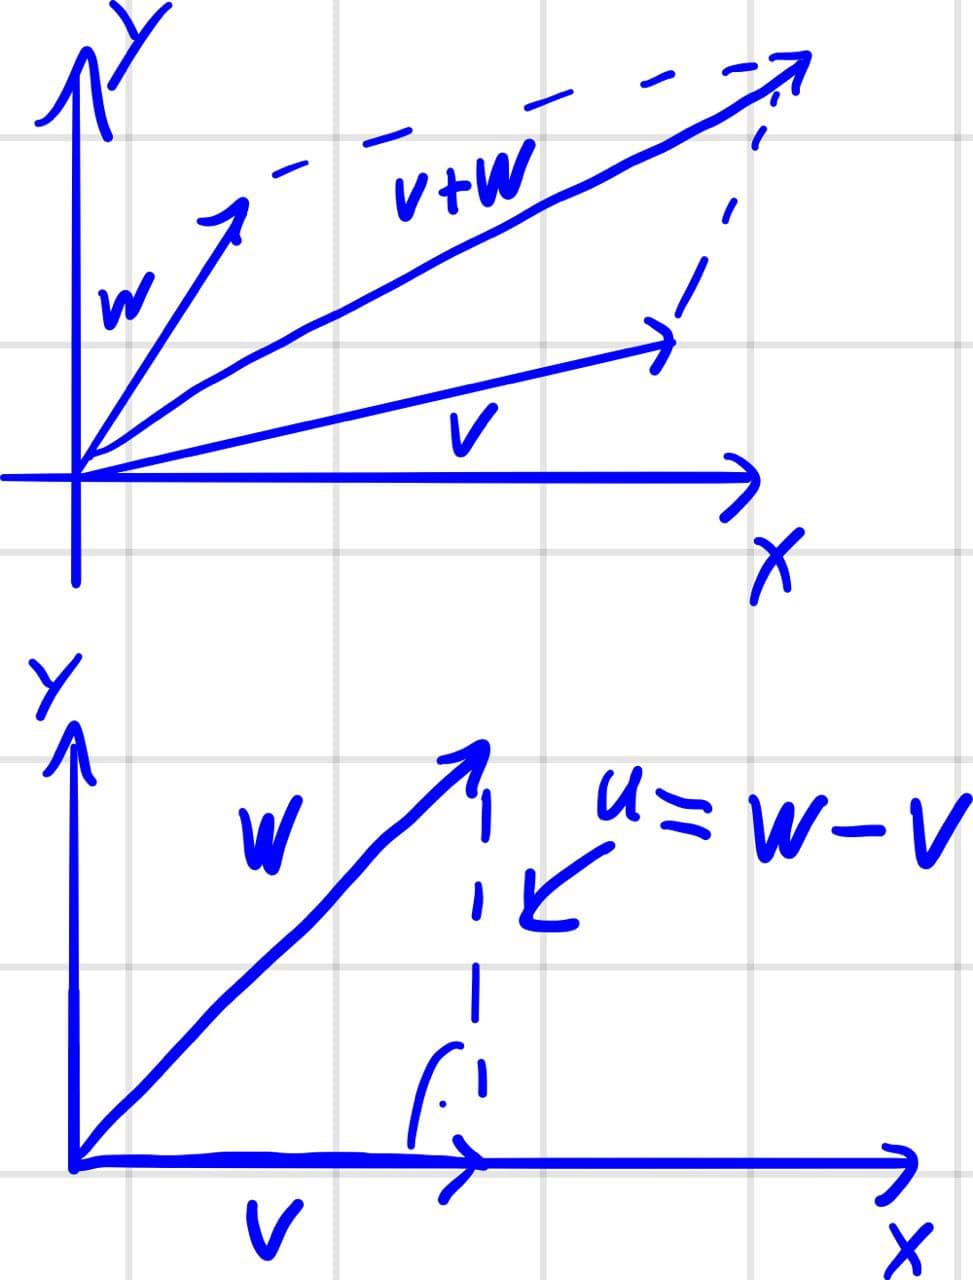
\includegraphics[width=.15\textwidth]{Dateien/04/04Vektoraddition.jpg}
 \vspace{-15pt}
\end{wrapfigure}
Geometrisch kann im $\mathbb{R}^2$ die Summe zweier Vektoren gewonnen werden, indem ein Parallelogramm gezeichnet wird.\\
Somit ist die Differenz zweier Vektoren quasi die dritte Seite eines Dreiecks.\\
Falls wir also wissen, dass $\vvec$ die orthogonale Projektion\footnote{welche wir mithilfe des Skalarprodukts gewinnen können} von $\wvec$ auf die bisherige Basis ist, erhalten wir durch $\vvec+\uvec=\wvec\iff \uvec=\wvec-\vvec$ einen zu $\vvec$ orthogonalen Vektor (siehe Skizze).
\end{Wiederholung}
\begin{Satz}{Kochrezept}{Gram-Schmidt-Verfahren}
\blue{Wir starten mit einer vorgegebenen Basis $B=(\textcolor{blue}{\vvec_1},\textcolor{blue}{\vvec_2},\ldots,\vvec_n)$ in einem euklidischen Vektorraum mit vorgegebenen Skalarprodukt.}\\
\red{Das Ziel ist eine orthonormale Basis $B'=(\textcolor{red}{\wvec_1},\textcolor{red}{\wvec_2},\ldots,\textcolor{red}{\wvec_n})$.}\\
So gehen wir vor:
\begin{enumerate}
	\item Wir fangen mit einem beliebigen Vektor, z. B. $\textcolor{blue}{\vvec_1}$, aus $B$ an und normieren diesen. Das ist schon der erste Vektor der neuen Basis:
	\begin{equation}
	\boxed{\textcolor{red}{\wvec_1}=\frac{\textcolor{blue}{\vvec_1}}{\Norm{\textcolor{blue}{\vvec_1}}}}.
	\end{equation}
	\item Falls die Basis $B'$ an dieser Stelle\footnote{Da man häufig zu diesem Schritt zurückkommt, tun wir so, als hätten wir schon $k$ orthonormale Basisvektoren gefunden. Das ist vielleicht anfangs ein wenig verwirrend, aber ergibt nach Schritt 5 mehr Sinn. Im Zweifel könnt ihr zunächst einfach $k=1$ betrachten :)} noch nicht orthogonal ist, konstruieren wir die \underline{orthogonale Projektion} $\textcolor{orange}{\Tilde{\vvec}_{k+1}}$ aus den bisher gewonnenen Basisvektoren $(\textcolor{red}{\wvec_1},\ldots,\textcolor{red}{\wvec_k})$ und dem nächsten Vektor $\vvec_{k+1}$ aus $B$:
	\begin{equation}
		\boxed{\textcolor{orange}{\Tilde{\vvec}_{k+1}}=\BiFo{\textcolor{blue}{\vvec_{k+1}},\textcolor{red}{\wvec_1}}\textcolor{red}{\wvec_1}+\ldots+\BiFo{\textcolor{blue}{\vvec_{k+1}},\textcolor{red}{\wvec_k}}\textcolor{red}{\wvec_k}}.
	\end{equation}
	Für den zweiten Basisvektor ist dies einfach
	\begin{equation*}
	    \textcolor{orange}{\Tilde{\vvec}_2}=\BiFo{\textcolor{blue}{\vvec_2},\textcolor{red}{\wvec_1}}\textcolor{red}{\wvec_1}.
	\end{equation*}
	\item Durch Subtraktion kann nun die Richtung des nächsten Basisvektors ermittelt werden, da so alle bisherigen Komponenten der Basis abgezogen werden:
	\begin{equation}
		\boxed{\textcolor{mygreen}{\Tilde{\wvec}_{k+1}}=\textcolor{blue}{\vvec_{k+1}}-\textcolor{orange}{\Tilde{\vvec}_{k+1}}}.
	\end{equation}
	Für den zweiten Basisvektor ist dies einfach
	\begin{equation*}
	    \textcolor{mygreen}{\Tilde{\wvec}_2}=\textcolor{blue}{\vvec_2}-\textcolor{orange}{\Tilde{\vvec}_2}.
	\end{equation*}
	\item Nun müssen wir diesen nur noch Normieren:
	\begin{equation}
	    \boxed{\textcolor{red}{\wvec_{k+1}}=\frac{\textcolor{mygreen}{\Tilde{\wvec}_{k+1}}}{\Norm{\textcolor{mygreen}{\Tilde{\wvec}_{k+1}}}}}.
	\end{equation}
	Für den zweiten Basisvektor ist dies einfach
	\begin{equation*}
	\textcolor{red}{\wvec_{2}}=\frac{\textcolor{mygreen}{\Tilde{\wvec}_{2}}}{\Norm{\textcolor{mygreen}{\Tilde{\wvec}_{2}}}}.
	\end{equation*}
	\item Nun müsst ihr die Schritte 2 bis 5 für den nächsten Vektor aus $B$ wiederholen, bis $B'$ vollständig orthonormal ist, ihr also alle $\textcolor{blue}{\vvec_i}$ verarbeitet habt.
\end{enumerate}
\end{Satz}
\begin{center}
    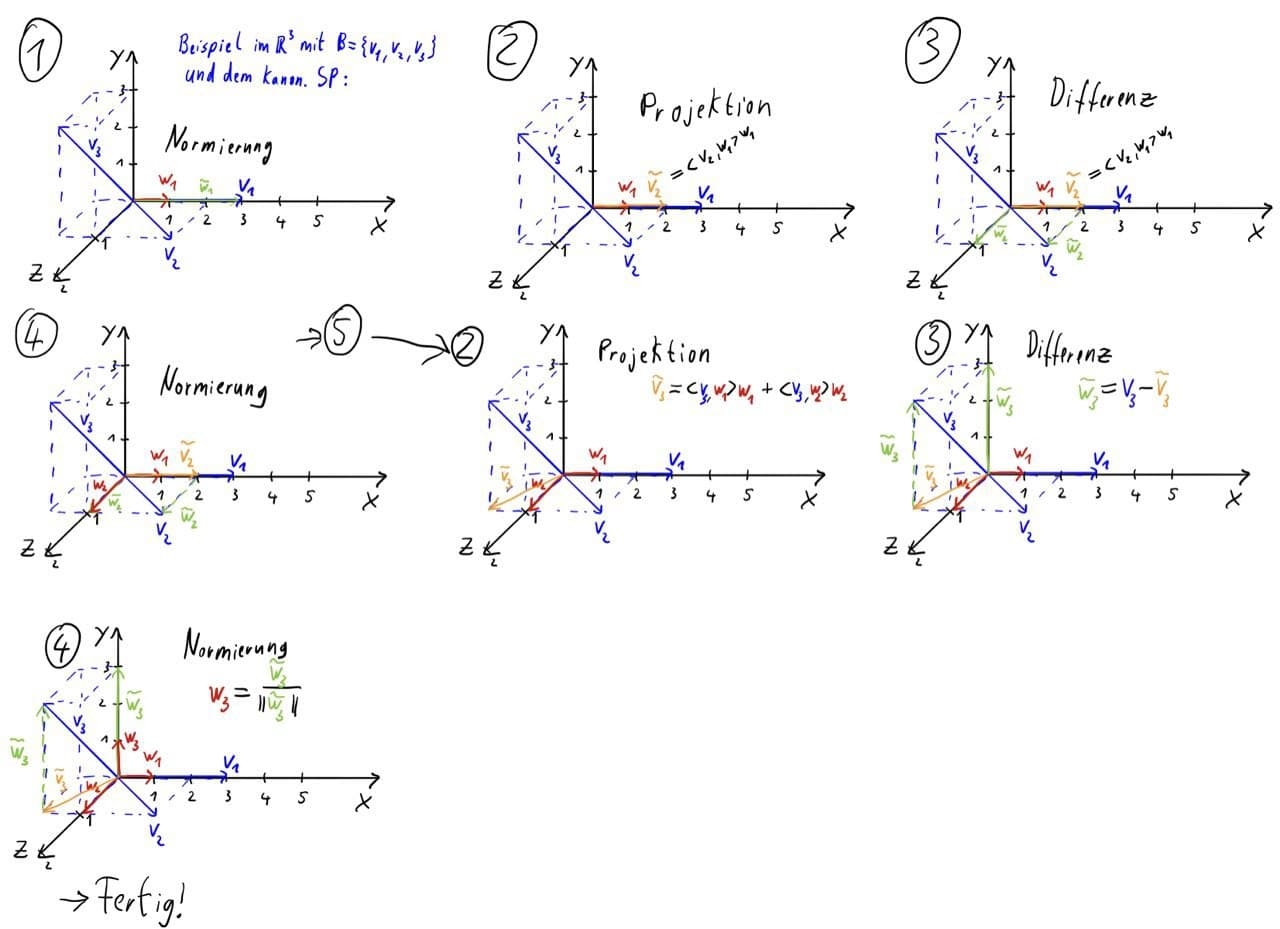
\includegraphics[width=\textwidth]{Dateien/03/03GramSchmidt.jpg}
\end{center}
In diesem Schaubild haben wir versucht, das Gram-Schmidt-Verfahren im $\mathbb{R}^3$ anschaulich darzustellen.

\begin{Beispiel}
{Anwendung des Gram-Schmidt-Verfahrens (1/2)}
Wir betrachten den $\mathbb{R}^3$ dem folgenden euklidischen Skalarprodukt:
\begin{equation*}
    \delta:\mathbb{R}^3\times \mathbb{R}^3\to\mathbb{R},\\
    \delta(\xvec,\yvec):=\BiFo{\xvec,\yvec}=4x_1y_1-2x_1y_2-2x_2y_1+4x_2y_2+x_3y_3+ x_3y_2+x_2y_3.
\end{equation*}
Bezüglich der kanonischen Basis $\hat{B}$ ist die darstellende Matrix dann
\begin{equation*}
    \Delta:=\Matrix{4&-2&0\\-2&4&1\\0&1&1}.
\end{equation*}
\blue{Wir sehen auch direkt, dass die Matrix symmetrisch ist. Tatsächlich ist sie auch positiv definit.\footnote{Es gibt Methoden, dies aus der Matrix abzulesen. Darauf möchten wir hier aber nicht eingehen. Es reicht nicht, dass $\det A>0$ ist! Dies ist aber trotzdem ein notwendiges Kriterium.}}\\
Wie würde nun eine ONB bezüglich dieses Skalarproduktes aussehen?\\
Wir fangen mit der kanonischen Basis $\hat{B}=\MengeDirekt{\MatrixInline{1\\0\\0},\MatrixInline{0\\1\\0},\MatrixInline{0\\0\\1}}=:\MengeDirekt{\textcolor{blue}{\vvec_1},\textcolor{blue}{\vvec_2},\textcolor{blue}{\vvec_3}}$ an und wählen $\textcolor{blue}{\vvec_1}$ als ersten Vektor:
\begin{enumerate}
    \item Die Länge von $\textcolor{blue}{\vvec_1}$ müssen wir nun\footnote{wahrscheinlich recht ungewohnt} bzgl. $\delta$ bestimmen, wir haben also
    \begin{equation*}
        \Norm{\textcolor{blue}{\vvec_1}}=\sqrt{\BiFo{\textcolor{blue}{\vvec_1},\textcolor{blue}{\vvec_1}}}=\sqrt{\Matrix{1&0&0}\Matrix{4&-2&0\\-2&4&1\\0&1&1}\Matrix{1\\0\\0}}=\sqrt{4}=2.
    \end{equation*}
    \red{Die Länge des kanonischen Einheitsvektors ist also bzgl. dieses Skalarproduktes nicht 1!}\\
    Somit legen wir fest:
    \begin{equation*}
        \textcolor{red}{\wvec_1}=\frac{\textcolor{blue}{\vvec_1}}{\Norm{\textcolor{blue}{\vvec_1}}}=\frac{1}{2}\Matrix{1\\0\\0}.
    \end{equation*}
    \item Wir projizieren $\textcolor{blue}{\vvec_2}$ auf $\textcolor{red}{\wvec_1}$:
    \begin{align*}
        \textcolor{orange}{\Tilde{\vvec}_2}&=\BiFo{\textcolor{blue}{\vvec_2},\textcolor{red}{\wvec_1}}\textcolor{red}{\wvec_1}=\Matrix{0&1&0}\Matrix{4&-2&0\\-2&4&1\\0&1&1}\Matrix{1/2\\0\\0}\textcolor{red}{\wvec_1}\\
        &=\Matrix{0&1&0}\Matrix{2\\-1\\0}\textcolor{red}{\wvec_1}=-1\textcolor{red}{\wvec_1}
    \end{align*}
    \item Wir ziehen die bisherigen Basiskomponenten ab:
    \begin{equation*}
        \textcolor{mygreen}{\Tilde{\wvec}_2}=\textcolor{blue}{\vvec_2}-\textcolor{orange}{\Tilde{\vvec}_2}=\Matrix{0\\1\\0}-\BracedIn{-\frac{1}{2}}\Matrix{1\\0\\0}=\Matrix{1/2\\1\\0}.
    \end{equation*}
    \item Abschließend normieren wir:
    \begin{align*}
        \Norm{\textcolor{mygreen}{\Tilde{\wvec}_2}}&=\sqrt{\Matrix{1/2&1&0}\Matrix{4&-2&0\\-2&4&1\\0&1&1}\Matrix{1/2\\1\\0}}=\sqrt{\Matrix{1/2&1&0}\Matrix{0\\3\\0}}=\sqrt{3}\\
        \implies \textcolor{red}{\wvec_2}&=\frac{\textcolor{mygreen}{\Tilde{\wvec}_2}}{\Norm{\textcolor{mygreen}{\Tilde{\wvec}_2}}}=\frac{1}{2\sqrt{3}}\Matrix{1\\2\\0}.
    \end{align*}
    \item Weil wir noch nicht alle Basisvektoren verarztet haben, kehren wir mit $\textcolor{blue}{\vvec_3}$ zu Schritt 2 zurück:\setcounter{enumi}{1}
    \item Wir projizieren $\textcolor{blue}{\vvec_3}$ auf die bisher gefundenen Basisvektoren $\textcolor{red}{\wvec_1}$ und $\textcolor{red}{\wvec_2}$:\footnote{Nebenrechnung: $\BiFo{\textcolor{blue}{\vvec_3},\textcolor{red}{\wvec_1}}=\textcolor{blue}{\vvec_3}^T \Delta \textcolor{red}{\wvec_1}=0$ und $\BiFo{\textcolor{blue}{\vvec_3},\textcolor{red}{\wvec_2}}=\textcolor{blue}{\vvec_3}^T\Delta \textcolor{red}{\wvec_2}=\frac{1}{2\sqrt{3}}\Matrix{0&0&1}\Matrix{0\\6\\2}=\frac{1}{\sqrt{3}}$.}
    \begin{equation*}
        \textcolor{orange}{\Tilde{\vvec}_3}=\BiFo{\textcolor{blue}{\vvec_3},\textcolor{red}{\wvec_1}}\textcolor{red}{\wvec_1}+\BiFo{\textcolor{blue}{\vvec_3},\textcolor{red}{\wvec_2}}\textcolor{red}{\wvec_2}=0\textcolor{red}{\wvec_1}+\frac{1}{\sqrt{3}}\textcolor{red}{\wvec_2}.
    \end{equation*}
    \item Wir ziehen die Projektion von $\textcolor{blue}{\vvec_3}$ ab:
    \begin{equation*}
        \textcolor{mygreen}{\Tilde{\wvec}_3}=\textcolor{blue}{\vvec_3}-\textcolor{orange}{\Tilde{\vvec}_3}=\Matrix{0\\0\\1}-\frac{1}{\sqrt{3}}\frac{1}{2\sqrt{3}}\Matrix{1\\2\\0}=\Matrix{-1/6\\-2/6\\1}=\frac{1}{6}\Matrix{-1\\-2\\6}.
    \end{equation*}
    \item Abschließend normieren wir:
    \begin{align*}
        \Norm{\textcolor{mygreen}{\Tilde{\wvec}_3}}&=\sqrt{\textcolor{mygreen}{\Tilde{\wvec}_3}^T\Delta \textcolor{mygreen}{\Tilde{\wvec}_3}}=\frac{1}{6}\sqrt{\Matrix{-1&-2&6}\Matrix{0\\-6\\4}}=\frac{1}{6}36=6\\
    \implies \textcolor{red}{\wvec_3}&=\frac{\textcolor{mygreen}{\Tilde{\wvec}_3}}{\Norm{\textcolor{mygreen}{\Tilde{\wvec}_3}}}=\frac{1}{36}\Matrix{-1\\-2\\6}.  
    \end{align*}
\end{enumerate}
Bezüglich des $\delta$-Skalarproduktes ist also $B'=\MengeDirekt{\frac{1}{2}\MatrixInline{1\\0\\0},\frac{1}{2\sqrt{3}}\MatrixInline{1\\2\\0},\\\frac{1}{36}\MatrixInline{-1\\-2\\6}}$ eine Orthonormalbasis!
\end{Beispiel}

\begin{Beispiel}
{Anwendung des Gram-Schmidt-Verfahrens (2/2)}
Wir suchen erneut eine orthogonale Basis bzgl. eines exotischen Skalarproduktes:
Für $\xvec,\yvec\in\mathbb{R}^3$ definieren wir das Skalarprodukt
\begin{equation*}
    \BiFo{\xvec,\yvec}=x_1y_1+2x_2y_2+3x_3y_3-x_2y_1-x_1y_2.
\end{equation*}
Wir beginnen mit der Basis $B:=\MengeDirekt{\MatrixInline{1\\1\\0},\MatrixInline{0\\1\\0},\MatrixInline{0\\0\\1}}=\MengeDirekt{\textcolor{blue}{\bvec_1},\textcolor{blue}{\bvec_2},\textcolor{blue}{\bvec_3}}$ und fordern, dass $\textcolor{blue}{\bvec_1}$ normiert in $B'$ enthalten ist.\\
Um uns das Leben leichter zu machen, stellen wir zunächst die darstellende Matrix $A$ von $\BiFo{\cdot,\cdot}$ bzgl. der kanonischen Basis auf:
\begin{equation*}
    A=\Matrix{1&-1&0\\-1&2&0\\0&0&3}.
\end{equation*}
Diese Matrix ist symmetrisch und positiv definit.
\begin{enumerate}
    \item Die Länge von $\textcolor{blue}{\bvec_1}$ ist
    \begin{align*}
        \Norm{\textcolor{blue}{\bvec_1}}&=\sqrt{\BiFo{\textcolor{blue}{\bvec_1},\textcolor{blue}{\bvec_1}}}=\sqrt{\textcolor{blue}{\bvec_1}^TA\textcolor{blue}{\bvec_1}}\\
        &=\sqrt{\Matrix{1&1&0}\Matrix{1&-1&0\\-1&2&0\\0&0&3}\Matrix{1\\1\\0}}=\sqrt{\Matrix{1&1&0}\Matrix{0&1&0}}=1.
    \end{align*}
    Somit legen wir fest:
    \begin{equation*}
        \textcolor{red}{\wvec_1}=\frac{\textcolor{blue}{\bvec_1}}{\Norm{\textcolor{blue}{\bvec_1}}}=\Matrix{1\\1\\0}.
    \end{equation*}
    \item Wir projizieren $\textcolor{blue}{\bvec_2}$ auf $\textcolor{red}{\wvec_1}$:
    \begin{equation*}
        \textcolor{orange}{\Tilde{b}_2}=\BiFo{\textcolor{blue}{\bvec_2},\textcolor{red}{\wvec_1}}\textcolor{red}{\wvec_1}=(\textcolor{blue}{\bvec_2}^T A \textcolor{red}{\wvec_1})\textcolor{red}{\wvec_1}=\Matrix{1\\1\\0}.
    \end{equation*}
    \item Wir ziehen die bisherigen Basiskomponenten ab:
    \begin{equation*}
        \textcolor{mygreen}{\Tilde{\wvec}_2}=\textcolor{blue}{\bvec_2}-\textcolor{orange}{\Tilde{b}_2}=\Matrix{-1\\0\\0}.
    \end{equation*}
    \item Abschließend normieren wir:\footnote{Es ist $\Norm{\textcolor{mygreen}{\Tilde{\wvec}_2}}=1$.}
    \begin{equation*}
        \textcolor{red}{\wvec_2}=\frac{\textcolor{mygreen}{\Tilde{\wvec}_2}}{\Norm{\textcolor{mygreen}{\Tilde{\wvec}_2}}}=\Matrix{-1\\0\\0}.
    \end{equation*}
    \item Weil wir noch nicht alle Basisvektoren verarztet haben, kehren wir mit $\textcolor{blue}{\vvec_3}$ zu Schritt 2 zurück:\setcounter{enumi}{1}
    \item Wir projizieren $\textcolor{blue}{\bvec_3}$ auf die bisher gefundenen Basisvektoren $\textcolor{red}{\wvec_1}$ und $\textcolor{red}{\wvec_2}$:\footnote{Nebenrechnung: $\BiFo{\textcolor{blue}{\bvec_3},\textcolor{red}{\wvec_1}}=\textcolor{blue}{\bvec_3}^T \Delta \textcolor{red}{\wvec_1}=0$ und $\BiFo{\textcolor{blue}{\bvec_3},\textcolor{red}{\wvec_2}}=0$.}
    \begin{equation*}
        \textcolor{orange}{\Tilde{b}_3}=\Matrix{0\\0\\0}.
    \end{equation*}
    \item Wir ziehen die Projektion von $\textcolor{blue}{\bvec_3}$ ab:
    \begin{equation*}
        \textcolor{mygreen}{\Tilde{\wvec}_3}=\textcolor{blue}{\bvec_3}-\textcolor{orange}{\Tilde{b}_3}=\Matrix{0\\0\\1}.
    \end{equation*}
    \item Abschließend normieren wir:
    \begin{align*}
        \Norm{\textcolor{mygreen}{\Tilde{\wvec}_3}}&=\sqrt{\textcolor{mygreen}{\Tilde{\wvec}_3}^T\Delta \textcolor{mygreen}{\Tilde{\wvec}_3}}=3\\
    \implies \textcolor{red}{\wvec_3}&=\frac{1}{3}\Matrix{0\\0\\1}.
    \end{align*}
\end{enumerate}
\end{Beispiel}

\subsection{Hermitesche Formen: Bilinearformen in komplex}
\blue{In diesem Kapitel werdet ihr oft den Satz 'Analog zu euklidischen Vektorräumen definieren wir...' finden, aber es gibt ein paar Feinheiten.\\
Wir erweitern zunächst das Konzept der Bilinearform auf komplexe Vektorräume:}
\begin{Def}
{Hermitesche Form}
Wir nennen\footnote{auf einem komplexen Vektorraum $V$} eine Abbildung $\BiFo{\cdot,\cdot}:V\times V\to\mathbb{C}$ \red{hermitesch} bzw. eine \red{hermitesche Form}, wenn sie $\mathbb{C}$-linear im ersten Argument ist und zudem $\forall \vvec,\wvec\in V$ gilt:
\begin{equation}
    \boxed{\overline{\BiFo{\vvec,\wvec}}=\BiFo{\wvec,\vvec}}.
\end{equation}
\blue{Sie muss also eine Art \textit{komplexe Symmetrie} erfüllen.}
\end{Def}
Folgende Definition liegt für komplexe Vektorräume auf der Hand:
\begin{Def}
{Konjugierte Linearität}
Eine Abbildung $F:V\to W$ zwischen komplexen Vektorräumen heißt \red{konjugiert linear}, wenn
\begin{equation}
    F(\vvec+\wvec)=F(\vvec)+F(\wvec)\quad\tx{und}\quad F(\lambda \vvec)=\overline{\lambda}F(\vvec)\quad\forall \vvec, \wvec\in V,\,\forall\lambda\in \mathbb{C}.
\end{equation}
\end{Def}
\blue{Aus der Linearität im ersten Argument und der Symmetriebedingung folgt, dass hermitesche Formen konjugiert linear im zweiten Argument sind: $\forall \uvec,\vvec,\wvec\in V,\lambda\in\mathbb{C}$ gilt:
\begin{equation*}
    \BiFo{\uvec,\lambda \vvec+\wvec}\overset{\footnotemark}{=}\overline{\lambda}\BiFo{\uvec,\vvec}+\BiFo{\uvec,\wvec}.
\end{equation*}\footnotetext{Denn $\BiFo{\uvec,\lambda \vvec+\wvec}=\overline{\BiFo{\lambda \vvec+\wvec, \uvec}}=\overline{\lambda\BiFo{\vvec,\uvec}+\BiFo{\wvec,\uvec}}=\overline{\lambda}\BiFo{\uvec,\vvec}+\BiFo{\uvec,\wvec}$, wobei wir die komplexe Symmetrie und die Linearität im 1. Argument genutzt haben.}Zudem ist $\BiFo{\vvec,\vvec}\in\mathbb{R}\,\forall \vvec\in V$, weil $\BiFo{\vvec,\vvec}\overset{!}{=}\overline{\BiFo{\vvec,\vvec}}\implies \Im (\BiFo{\vvec,\vvec})=0$.}
\subsubsection{Komplexere Skalarprodukte}
Wie auch für das euklidische SP fordern wir noch die positive Definitheit für hermitesche SP. Diese ist wie folgt definiert:
\begin{Def}
{Positive Definitheit (Hermitesche Formen)}
Weil $\BiFo{\vvec,\vvec}$ reell ist, können wir die Ordnungsrelationen verwenden und analog zu Bilinearformen die \red{positive Definitheit} von hermiteschen Formen definieren:
\begin{equation}
    \BiFo{\cdot,\cdot}\tx{ pos. definit}\iff \BiFo{\vvec,\vvec}>0\quad\forall \vvec\in V\setminus\MengeDirekt{\Vec{0}}.
\end{equation}
\end{Def}
\begin{Def}
{Hermitesches Skalarprodukt}
Eine \underline{positiv definite hermitesche Form} $\BiFo{\cdot,\cdot}: V\times V\to \mathbb{C}$ nennen wir \red{hermitesches Skalarprodukt}.
\end{Def}
\begin{Def}
{Hermitescher Vektorraum}
Einen komplexen Vektorraum nennen wir \red{hermitesch} oder auch \red{unitär}, falls für ihn ein hermitesches Skalarprodukt definiert ist.
\end{Def}
\begin{Beispiel}
{Kanonisches Skalarprodukt}
Auf $\mathbb{C}^n$ ist durch $\BiFo{\cdot,\cdot}:\mathbb{C}^n\times \mathbb{C}^n\to\mathbb{C},\,(\vvec,\wvec)\mapsto \BiFo{\vvec,\wvec}=\sum_{i=1}^n\vvec_i\overline{\wvec_i}$ das kanonische hermitesche Skalarprodukt definiert.
\end{Beispiel}

\begin{Def}
{Norm von Vektoren und die Cauchy-Schwarzsche Ungleichung}
Analog zu euklidischen Vektorräumen definieren wir die \red{Norm} bzw. \red{Länge} eines Vektors $v\in V$ (wobei $V$ ein herm. VR ist) als
\begin{equation}
    \Norm{\vvec}:=\sqrt{\BiFo{\vvec,\vvec}}
\end{equation}
und es gilt
\begin{equation}
    \Abs{\BiFo{\vvec,\wvec}}\leq \Norm{\vvec}\cdot\Norm{\wvec}\quad \forall \vvec,\wvec\in V.
\end{equation}
\end{Def}

\subsubsection{Unitarität ist die komplexe Orthogonalität}
\begin{Def}
{Unitäre Basis}
Analog zur orthogonalen Basis für euklidische Vektorräume nennen wir die Basis $B$ eines herm. Vektorraums $V$ \red{unitär}, wenn
\begin{equation}
\BiFo{\wvec_i,\wvec_j}=\delta_{ij}\quad\forall \wvec_i, \wvec_j\in B.
\end{equation}
\end{Def}
\begin{Satz}
{Satz}{Existenz einer unitären Basis}
Auch hier kann man zeigen, dass jeder hermitesche Vektorraum eine Basis besitzt.
\end{Satz}

\subsection{Klassifikation von Endomorphismen}
\blue{Wir betrachten nun wieder Endomorphismen\footnote{diesmal auf euklidischen oder hermiteschen Vektorräumen} und schauen uns Eigenschaften an, die wir mithilfe eines Skalarproduktes überprüfen können.}

\subsubsection{Orthogonale und unitäre Endomorphismen}
\blue{Die ersten Kandidaten dafür sind Abbildungen, welche Winkelbeziehungen, Längen und Abstände von Vektoren erhalten:}
\begin{Def}
{Orthogonale Endomorphismen}
Auf einem euklidischen Vektorraum $V,\BiFo{\cdot,\cdot})$ nennen wir eine \underline{surjektive} lineare Abbildung $F:V\to V$ \red{orthogonal}, wenn gilt
\begin{equation}
    \boxed{\BiFo{F(\vvec),F(\wvec)}=\BiFo{\vvec,\wvec}}\quad \forall \vvec,\wvec\in V.
\end{equation}
\end{Def}
\blue{Aufgrund der Bedingung ist $F$ \underline{stets injektiv}, denn\\ $F(\vvec)=0\implies \vvec=0$, weil ja $0=\BiFo{F(\vvec),F(\vvec)}=\BiFo{\vvec,\vvec}$.\\
Auf endlichdimensionalen Vektorräumen ist $F$ aufgrund der Dimensionsformel dann auch surjektiv. So oder so ist $F$ stets ein \underline{bijektiver Endomorphismus}, was wir ja auch als \underline{Automorphismus} bezeichnen.}
\begin{Def}
{Orthogonale Gruppe}
Es gilt: $O(V)\subseteq \Aut(V)$, d. h. die \red{orthogonale Gruppe\footnote{diese beinhaltet alle orthogonalen Endomorphismen von $V$} $O(V)$} ist eine Untergruppe der Automorphismen.
\end{Def}
\begin{Satz}
{Satz}{Matrizen orthogonaler Endomorphismen im $\mathbb{R}^n$}
Im $\mathbb{R}^n$ gilt mit dem kanonischen Skalarprodukt, dass $O(n):=O(\mathbb{R}^n,\BiFo{\cdot,\cdot})$ der Gruppe \red{invertierbarer Matrizen} entspricht, für die
\begin{equation}
    A^{-1}=A^T \iff A^T A=\mathds{1}_n.
\end{equation}
\end{Satz}
\begin{Def}
{Unitäre Endomorphismen}
Analog dazu bezeichnet man surjektive lineare Abbildungen $F:V\to V$ auf hermiteschen Vektorräumen $V$ als \red{unitär}, wenn
\begin{equation}
    \boxed{\BiFo{F(\vvec),F(\wvec)}=\BiFo{\vvec,\wvec}}\quad \forall \vvec,\wvec\in V.
\end{equation}
\end{Def}
\blue{Auch hier folgt wieder die Injektivität direkt und die Surjektivität muss für $\dim V<\infty$ nicht gefordert werden. Die \red{unitäre Gruppe} ist ebenfalls eine Untergruppe der Automorphismen, $U(V)\subseteq \Aut(V)$.}
\begin{Def}
{Notation: $A$ Dagger}
Wir definieren das gleichzeitige komplexe Konjugieren und Transponieren einer Matrix $A\in\mathbb{C}^n$ mit dem folgenden Zeichen: $A^\dag:=\overline{A}^T=\overline{A^T}$ (sprich: 'A dagger').
\end{Def}
\begin{Satz}
{Matrizen unitärer Endomorphismen im $\mathbb{C}^n$}
Im $\mathbb{C}^n$ gilt mit dem kanonischen Skalarprodukt $\BiFo{\wvec,\zvec}=\sum_{i=1}^nw_i\overline{z_i}$, dass $U(n):=U(\mathbb{C}^n,\BiFo{\cdot,\cdot})$ der Gruppe \red{invertierbarer Matrizen} entspricht, für die
\begin{equation}
    A^{-1}=A^\dag \iff A^\dag A=\mathds{1}_n.
\end{equation}
\end{Satz}
Unitäre Matrizen sind in der Physik unglaublich wichtig - z. B. lernt ihr in Physik 5 die \href{https://de.wikipedia.org/wiki/CKM-Matrix}{CKM-Matrix} kennen, die essenzieller Bestandteil des heutigen Standardmodells der Teilchenphysik ist.\\
Ein anschauliches Beispiel ist die euch bekannte Drehmatrix:
\begin{Beispiel}
{Drehmatrix}
Im $\mathbb{R}^2$ ist die Drehmatrix $D_\varphi=\MatrixInline{\cos\varphi&-\sin\varphi\\\sin\varphi&\cos\varphi}$ ein orthogonaler Endomorphismus, denn es gilt
\begin{align*}
    D_\varphi^TD_\varphi&=\Matrix{\cos\varphi&\sin\varphi\\-\sin\varphi&\cos\varphi}\Matrix{\cos\varphi&-\sin\varphi\\\sin\varphi&\cos\varphi}\\
    &=\Matrix{\cos^2\varphi-(-\sin^2\varphi)&\cos\varphi\sin\varphi-\cos\varphi\sin\varphi\\0&\cos^2\varphi+\sin^2\varphi}=\Matrix{1&0\\0&1}=\mathds{1}_2.
\end{align*}
\textbf{Alternativer Beweis}:\\
Für $\vvec,\wvec\in\mathbb{R}^2,\vvec:=\MatrixInline{a\\b}, \wvec:=\MatrixInline{c\\d}$ gilt
\begin{align*}
    \BiFo{D_\varphi \vvec,D_\varphi \wvec}&=\BiFo{\Matrix{a\cos\varphi-b\sin\varphi\\a\sin\varphi+b\cos\varphi},\Matrix{c\cos\varphi-d\sin\varphi\\c\sin\varphi+d\cos\varphi}}\\
    &=ac\cos\varphi^2-ad\cos\varphi\sin\varphi-bc\cos\varphi\sin\varphi+bd\sin\varphi^2+ac\cos\varphi^2\\
    &\quad +ad\cos\varphi\sin\varphi+bc\cos\varphi\sin\varphi+bd\sin\varphi^2\\
    &=ac(\cos^2\varphi+\sin^2\varphi)+bd(\sin^2\varphi+\cos^2\varphi)=ac+bd\\
    &=\BiFo{\Matrix{a\\b},\Matrix{c\\d}}=\BiFo{\vvec,\wvec}.
\end{align*}
\end{Beispiel}

\subsubsection{Diagonalisierung orthogonaler/unitärer Endomorphismen}
Die darstellenden Matrizen orthogonaler bzw. unitärer Endomorphismen sind in besonderer Weise diagonalisierbar.\\
Aufgrund der Eigenschaft, Längen von Vektoren zu erhalten, haben die Eigenwerte stets den Betrag 1.\footnote{Kurze Übungsaufgabe: Könnt ihr zeigen, dass für unitäre Matrizen $U$ stets $\Abs{\det U}=1$ gilt?\\
Für solche Matrizen ist $U^\dag U=\mathds{1}_n$, woraus folgt, dass $1=\det\mathds{1}_n=\det(U^\dag U)=\det U^\dag \det U=\overline{\det U^T}\det U=\Abs{\det U}^2$, wobei wir den Determinantenmultiplikationsatz und $\det A^T=\det A$ genutzt haben.
}
Zudem hat die Basis des Vektorraumes, bzgl. derer diese Diagonalgestalt erreicht wird, besondere Eigenschaften.
\begin{Satz}
{Satz}{Normalform orthogonaler (bzw. unitärer) Endomorphismen}
Auf euklidischen Vektorräumen $V$ mit $\dim V<\infty$ gilt für $F\in O(V)$:
\begin{enumerate}
    \item Eigenwerte von $F$ sind $+1$ oder $-1$.
    \item Eigenvektoren zu verschiedenen Eigenwerten stehen \underline{senkrecht} aufeinander.
    \item Es existiert eine \underline{Orthonormalbasis}, bzgl. derer die darst. Matrix $A_F$ die folgende Gestalt annimmt:
    \begin{equation}
        A_F=\diag\BracedIn{\lambda_1,\ldots,\lambda_p,D_{\varphi_1},\ldots,D_{\varphi_q}}
    \end{equation}
    mit $\lambda_j\in\MengeDirekt{-1,1}$ und $D_{\varphi_j}=\MatrixInline{\cos\varphi_j&-\sin\varphi_j\\\sin\varphi_j&\cos\varphi_j}$ mit $\phi_j\in\mathbb{R}$.\\
    Hierbei gilt, dass $p+2q=\dim V$.
\end{enumerate}
Auf hermiteschen, endlichdimensionalen Vektorräumen gilt analog für $F\in U(V)$:
\begin{enumerate}
    \item Eigenwerte $\lambda_i$ sind komplexe Zahlen mit $\Abs{\lambda_i}=1$.
    \item Eigenvektoren zu verschiedenen Eigenwerten sind unitär.
    \item Es existiert eine unitäre Basis, bzgl. derer $A_F$ die folgende Gestalt hat:
    \begin{equation}
        A_F=\diag(\lambda_1,...\lambda_n).
    \end{equation}
    Hier werden die $D_{\varphi_j}$ also nicht benötigt.
\end{enumerate}
\blue{Im komplexen ist $F$ bzgl. einer unitären Basis also komplett diagonalisierbar!}
\end{Satz}
Dass Eigenwerte den Betrag 1 haben müssen, ist mit der Eigenwertgleichung $F(\vvec)=\lambda \vvec$ leicht zu zeigen! Los, probiert es selbst!\\
\Zb{Aufgrund der positiven Definitheit wissen wir,\footnote{egal ob wir euklidische oder hermitesche Vektorräume betrachten} dass $\BiFo{\vvec,\vvec}>0$ für Eigenvektoren von $F$ gilt, da der $\Vec{0}$-Vektor per Definition kein Eigenvektor ist.\\
Es gilt mit der Eigenschaft der orthogonalen/unitären Endomorphismen für Eigenvektoren $\vvec$ von $F$ dann
\begin{equation}
    \BiFo{\vvec,\vvec}\overset{\footnotemark}{=}\BiFo{F(\vvec),F(\vvec)}\overset{\footnotemark}{=}\BiFo{\lambda \vvec,\lambda \vvec}\overset{\footnotemark}{=}\lambda\BiFo{\vvec,\lambda \vvec}=\overset{\footnotemark}{=}\lambda \overline{\lambda}\BiFo{\vvec,\vvec}=\Abs{\lambda}^2\BiFo{\vvec,\vvec}.
\end{equation}\footnotetext{Definition solcher Endomorphismen}\footnotetext{Eigenwert-Gleichung}\footnotetext{Linearität 1. Argument}\footnotetext{Konjugierte Linearität im 2. Argument (für reelle Zahlen ist dies ja egal).}Daraus folgt $1=\Abs{\lambda}^2\implies\Abs{\lambda}=1$.}

\subsubsection{Adjungierte Endomorphismen}
\blue{Wir können das Skalarprodukt auch ausnutzen, um eine weitere lustige Eigenschaft bzw. Beziehung zwischen Endomorphismen zu definieren:}
\begin{Def}
{Adjungiertheit von Endomorphismen}
Für einen Endomorphismus eines eukl. oder herm. Vektorraums $(V,\BiFo{\cdot,\cdot})$ nennen wir $F^\ad\in \End(V)$ den zu $F$ \red{adjungierten} Endomorphismus, wenn
\begin{equation}
    \BiFo{F(\vvec),\wvec}=\BiFo{\vvec,F^\ad(\wvec)}\quad\forall \vvec,\wvec\in V.
\end{equation}
\end{Def}
\begin{Satz}
{Satz}{Eindeutigkeit und Existenz von adj. Endomorphismen}
Es existiert höchstens \underline{ein} $F^\ad$ zu einem gegebenen Endomorphismus $F$.\\
Ist $\dim V<\infty$, so existiert $F^\ad$ für alle $F\in\End(V)$.
\end{Satz}
\begin{Def}
{Selbstadjungiertheite Endomorphismen}
Wir nennen $F\in\End(V)$ \red{selbstadjungiert}, falls $F=F^\ad$, d. h. $\BiFo{F(\vvec),\wvec}=\BiFo{\vvec,F(\wvec)}$ $\forall \vvec,\wvec\in V$.
\end{Def}
\begin{Def}
{Normale Endomorphismen}
Ist die Verknüpfung von $F$ mit $F^\ad$ kommutativ, d. h. $F^\ad\circ F=F\circ F^\ad$, so heißt $F$ \red{normal}.
\end{Def}
\begin{Satz}
{Satz}{Zur darst. Matrix adjungierter Endomorphismen bzgl. Orthonormalbasen}
Auf euklidischen oder hermiteschen Vektorräumen $V$ mit $\dim V<\infty$ ist für $F$ mit darstellender Matrix $A$ bezüglich einer Orthonormalbasis\footnote{bzw. unitären Basis} die darst. Matrix von $F^\ad$ gegeben durch $A^\dagger$.\\
Bzgl. einer solchen Basis gilt also:
\begin{equation}
    F\tx{ selbstadjungiert}\iff A=A^\dag.
\end{equation}
Im komplexen nennen wir eine Matrix $B$ mit $B=B^\dag$ \red{hermitesch}.\footnote{analog zur symmetrischen Matrix mit $B=B^T$.}
\end{Satz}
\blue{\textbf{Anmerkung}:\\
Die darst. Matrizen symmetrischer Bilinearformen bzw. von hermiteschen Formen haben genau diese Eigenschaft.}
\begin{Satz}{Satz}
{Eigenschaften selbstadjungierter Endomorphismen}
Für $F\in\End(V)$ mit $F=F^\ad$ gilt:
\begin{itemize}
    \item $F$ hat reelle Eigenwerte.\\
    \Zb{Sei $v$ ein Eigenvektor zu $\lambda$ mit $\Norm{\vvec}=1$, so ist
    \begin{equation*}
        \lambda=\lambda\BiFo{\vvec,\vvec}\overset{\footnote{Linearität 1. Argument und Eigenwertgleichung}}{=}\BiFo{F(\vvec),\vvec}\overset{\footnote{Selbstadjungiertheit}}{=}\BiFo{\vvec,F(\vvec)}\overset{\footnote{Eigenwertgleichung, konjugierte Linearität im 2. Argument}}{=}\overline{\lambda}\BiFo{\vvec,\vvec}=\overline{\lambda}.
    \end{equation*}}
    \item Eigenvektoren verschiedener Eigenwerte sind paarweise orthogonal.\\
    \Zb{Sei $\lambda$ Eigenwert zum Eigenvektor $\vvec$ und $\mu$ ein dazu verschiedener Eigenwert zum Eigenvektor $\wvec$, so gilt:
    \begin{equation*}
        \lambda\BiFo{\vvec,\wvec}=\BiFo{\lambda \vvec, \wvec}\overset{\footnote{Eigenwertgleichung}}{=}\BiFo{F(\vvec),\wvec}\overset{\footnote{Selbstadjungiertheit}}{=}\BiFo{\vvec,F(\wvec)}\overset{\footnote{Eigenwertgleichung und konjugierte Linearität}}{=}\overline{\mu}\BiFo{\vvec,\wvec}\overset{\footnote{$\mu$ ist reell}}{=}\mu \BiFo{\vvec,\wvec}.
    \end{equation*}
    Da per Voraussetzung $\lambda\neq \mu$, muss $\BiFo{\vvec,\wvec}=0$ sein, d. h. $\vvec\perp \wvec$.}
    \item Für $\dim V<\infty$ existiert stets eine orthogonale bzw. unitäre Basis von $V$, die aus den Eigenvektoren von $F$ besteht.
\end{itemize}
\end{Satz}

\begin{Satz}
{Satz}{Zur Isomophie und Dualisierung}
Für euklidische, endlichdimensionale Vektorräume ist der Raum der symmetrischen Bilinearformen \underline{isomorph}\footnote{d. h., dass eine bijektive lineare Abbildung existiert} zum Raum der selbstadjungierten Endomorphismen. 
\end{Satz}
\blue{Dies ergibt intuitiv auch Sinn, denn wir hatten gesehen, dass darstellende Matrizen symmetrischer Bilinearformen symmetrisch sind, also $A=A^T$. Auf euklidischen Vektorräumen ist dies für Endomorphismen ein Zeichen der Selbstadjungiertheit.}\\
Analog gilt der Satz auch für hermitesche Vektorräume mit hermiteschen Formen.
\subsubsection{Hauptachsentransformation - wenn Endomorphismen Signaturen hinterlassen}
\blue{Durch geschickte Reskalierung der Basisvektoren können wir (weil diese orthogonal sind) eine ganz besondere Form der darstellenden Matrix erhalten, die nur noch von den Vorzeichen der Eigenwerte abhängt.\\
Aufgrund der Isomorphie betrachten wir nun symmetrische Bilinearformen bzw. hermitesche Formen.}
\begin{Satz}
{Satz}{Hauptachsentransformation und Trägheitssatz von Sylvester}
Auf einem euklidischen Vektorraum $V$ mit $\dim V=n$ gilt für \underline{symmetrische} Bilinearformen $\beta$:
\begin{itemize}
    \item Es existiert eine \red{orthogonale Basis} $B=(\bvec_1,\ldots,\bvec_n)$ von $V$, bzgl. derer die darstellende Matrix die folgende Gestalt hat:
    \begin{equation}
        M_B(\beta)=\diag(\mathds{1}_{r_+},-\mathds{1}_{r_-},\Vec{0}_{r_0}).
    \end{equation}
    Hierbei gilt $\boxed{r_++r_-+r_0=n}$ und $\Vec{0}_{r_0}\in\Met(r_0,\mathbb{R})$ die $r_0\times r_0$-Nullmatrix.\\
    Eine solche Gestalt nennt man auch \red{Normalform}.
    \item Die Zahlen $r_+$, $r_-$ und $r_0$ hängen \underline{nicht} von der Wahl der Basis ab.\\
    Man nennt sie auch die \red{Signatur} von $\beta$.
\end{itemize}
Aufgrund der letzten Aussage sind $r_+$ und $r_-$ genau die Anzahl positiver bzw. negativer Eigenwerte.
\end{Satz}
\red{Achtung: $\beta$ muss kein Skalarprodukt sein und ist insbesondere nicht das Skalarprodukt des zugrunde liegenden euklidischen Vektorraums!}
\begin{Beispiel}
{Hauptachsentransformierte Matrix}
Seien $r_+=3$, $r_-=1$, $r_0=2$. Dann ist
\begin{equation*}
    A=\Matrix{1&0&0&0&0&0\\0&1&0&0&0&0\\0&0&1&0&0&0\\0&0&0&-1&0&0\\0&0&0&0&0&0\\0&0&0&0&0&0}
\end{equation*}
die hauptachsentransformierte Matrix auf einem Vektorraum der Dimension\\
$\dim V=3+1+2=6$.
\end{Beispiel}
\begin{Satz}
{Exkurs}{Finden der orthogonalen Basis (nicht im Skript)}\label{satz:04Hauptachsenbasis}
Sei auf einem eukl. VR $V$ eine symmetrische Bilinearform $\beta$ gegeben.\\
Wir suchen nun die orthogonale Basis $B$ von $V$, bzgl. derer die darst. Matrix von $\beta$ Normalform annimmt.\\
Um diese orthogonale Basis zu finden, müssen wir zunächst die Eigenvektoren $\wvec_i$ zu $\beta$ finden. Als Voraussetzung wissen wir ja immerhin, dass diese orthogonal sind.\\
\Zb{Seien $\bvec_i$ die orthogonalen Basisvektoren, die $\beta$ in Normalform bringen, und $\wvec_i$ weiterhin die Eigenvektoren.\\
Da die $\wvec_i$ bereits eine orthogonale Basis bilden, wählen wir $\bvec_i=c_i\wvec_i$ mit $c_i\in\mathbb{R}$, die neuen Basisvektoren müssen also nur noch richtig skaliert werden.\\
Die Frage ist also, wie diese Vorfaktoren gewählt werden müssen.\\
Die Einträge der darstellenden Matrix $\alpha_{ij}$ ergeben sich durch Anwenden der Bilinearform auf die Basisvektoren, $\alpha_{ij}=\beta(\bvec_i,\bvec_j)$.\\
In Normalform haben wir also $N=\MatrixInline{\beta(\bvec_1,\bvec_1)&\cdots& \alpha_{1n}\\\vdots&\ddots&\vdots\\\alpha_{n1}&\cdots&\alpha_{nn}}.$\\
Wir gucken uns das genauer an:
\begin{eqnarray*}
\alpha_{ij}&=&\beta(\bvec_i,\bvec_j)\\
&=&\beta(c_i\wvec_i, c_i\wvec_j)\\
&\overset{\footnote{$\beta$ ist bilinear}}{=}&c_ic_j\beta(\wvec_i,\wvec_j)\\
&\overset{\footnote{$A$ sei die darst. Matrix von $\beta$. Achtung: $\BiFo{\cdot,\cdot}$ ist das Skalarprodukt des eukl. Vektorraums!}}{=}&c_ic_j\BiFo{\wvec_i,A\wvec_j}\\
&\overset{\footnote{Eigenwertgleichung}}{=}&c_ic_j\BiFo{\wvec_i,\lambda_j\wvec_j}\\
&\overset{\footnote{Bilinearität}}{=}&\lambda_jc_ic_j\underbrace{\BiFo{\wvec_i,\wvec_j}}_{=\delta_{ij}\sqrt{\BiFo{\wvec_i,\wvec_j}}^2}\overset{\footnote{weil $\wvec_i$ und $\wvec_j$ als Eigenvektoren einer symmetrischen Bilinearform (isomorph zu selbstadjungierten Endomorphismen) paarweise orthogonal sind.}}{=}\Cases{0&\tx{ wenn } i\neq j\\\lambda_ic_i^2\Norm{\wvec_i}^2&\tx{ wenn } i=j}.
\end{eqnarray*}
Nun sollen aber die Einträge auf der Hauptdiagonalen $\alpha_{ii}$ genau 1, -1 oder 0 sein, also $\Abs{1}$ haben. Für $\lambda_i=0$ stellt sich heraus, dass die Skalierungsfaktoren $c_i$ der $\wvec_i$ egal sind.\\
Für $\lambda_i\neq0$ ergibt sich also:
\begin{equation}
    \sgn(\lambda_i)\cdot 1\overset{!}{=}\lambda_ic_i^2\Norm{\wvec_i}^2\iff \boxed{c_i=\frac{1}{\sqrt{\Abs{\lambda_i}}\Norm{\wvec_i}}}.
\end{equation}
Hierbei nutzten wir das Vorzeichen $\sgn(\lambda_i)$ und den Fakt, dass $\frac{\lambda_i}{\sgn(\lambda_i)}=\Abs{\lambda_i}$ ist. Beim Wurzelziehen haben wir die $c_i$ zudem positiv gewählt, dies ist aber willkürlich.\\
Somit sind die Basisvektoren für die Normalform gegeben durch
\begin{equation*}
    \boxed{\bvec_i=c_i\wvec_i=\Cases{\frac{\wvec_i}{\sqrt{\Abs{\lambda_i}}\Norm{\wvec_i}}&\lambda_i\neq0\\\wvec_i&\lambda_i=0}}.
\end{equation*}}
\end{Satz}

\begin{Satz}
{Satz}{Hauptachsentrafo auf komplexen Vektorräumen}
Für hermitesche Formen $h$ auf $\mathbb{C}$-Vektorräumen existiert ebenfalls eine Basis, bzgl. derer die darst. Matrix von $h$ die Normalform-Gestalt (d. h. $\diag(\mathds{1}_{r_+},-\mathds{1}_{r_-},\Vec{0}_{r_0})$).\\
Hierbei wird (im \Skript{}) aber keine Aussage über die Gestalt der Basis getroffen.\\
Ist $V$ hermitesch, so ist die Basis aber tatsächlich orthogonal.
\end{Satz}

\begin{Beispiel}
{Bestimmung der Signatur und der orthogonalen Basis einer hermiteschen Form}
Wir betrachten
\begin{equation*}
    \gamma:\mathbb{C}^2\times \mathbb{C}^2\to\mathbb{C},\quad \gamma(\vvec,\wvec):=\BiFo{\vvec,\Matrix{2&i\\-i&4}\wvec},
\end{equation*}
wobei $\BiFo{\cdot ,\cdot}$ das kanonische Skalarprodukt von $\mathbb{C}^2$ sei.\\
$\gamma$ ist eine hermitesche Form, denn $A=\MatrixInline{2&i\\-i&4}=\MatrixInline{2&-i\\i&4}^T=\overline{\MatrixInline{2&i\\-i&4}^T}=A^\dag$.\\
Wir suchen die Eigenwerte über das charakteristische Polynom:
\begin{equation*}
    P_A(\lambda)=(2-\lambda)(4-\lambda)+i^2=\lambda^2-6\lambda+7\implies \lambda_1=3+\sqrt{2},\,\lambda_2=3-\sqrt{2}.
\end{equation*}
Weil wir zwei positive Eigenwerte haben, ist die Signatur also\\
$(2,0,0):=r_+=2\land r_-=0\land r_0=0$.\\
Wir suchen nun die Eigenvektoren:
\begin{align*}
    A\wvec_1&=\lambda_1\wvec_1\iff \MatrixInvertieren{-1-\sqrt{2}&i\\-i&1-\sqrt{2}}{0\\0}\to\MatrixInvertieren{1+\sqrt{2}&-i\\1&i(1-\sqrt{2})}{0\\0}\\
    &=\MatrixInvertieren{1+\sqrt{2}&-i\\0&i(1-\sqrt{2})+\frac{i}{1+\sqrt{2}}}{0\\0}=\MatrixInvertieren{1+\sqrt{2}&-i\\0&\frac{i}{1+\sqrt{2}}(1^2-\sqrt{2}^2+1)}{0\\0}\\
    &=\MatrixInvertieren{1+\sqrt{2}&-i\\0&0}{0\\0}\implies y=t\in\mathbb{R}\implies x=\frac{it}{1+\sqrt{2}}
\end{align*}
Somit sind die Eigenvektoren ($\wvec_2$ analog)
\begin{equation*}
    \wvec_1=t\Matrix{\frac{i}{1+\sqrt{2}}\\1},\quad \wvec_2=t\Matrix{\frac{i}{\sqrt{2}-1}\\1}.
\end{equation*}
Diese Eigenvektoren sind orthogonal, denn (wir lassen den Skalierungsfaktor $t$ weg) 
\begin{equation*}
    \BiFo{\wvec_1,\wvec_2}=\sum_{i=1}^2\wvec_{1i}\overline{\wvec_{2i}}=\BracedIn{\frac{i}{1+\sqrt{2}}}\overline{\BracedIn{\frac{i}{\sqrt{2}-1}}}+1=\frac{1}{(1+\sqrt{2})(1-\sqrt{2})}+1=-1+1=0.
\end{equation*}
Wir können nun die unitären Basisvektoren $\bvec_i=\frac{\wvec_i}{\sqrt{\Abs{\lambda_i}}\Norm{\wvec_i}}$ bestimmen:
\begin{align*}
    \Norm{\wvec_1}&=\sqrt{\BiFo{\wvec_1,\wvec_1}}=\sqrt{\frac{i}{1+\sqrt{2}}\frac{-i}{1+\sqrt{2}}t^2+t^2}=t\frac{\sqrt{4+2\sqrt{2}}}{1+\sqrt{2}}=\frac{\sqrt{2(2+\sqrt{2})}(\sqrt{2}-1}{(1+\sqrt{2})(\sqrt{2}-1)}t\\
    &=\frac{\sqrt{2(2+\sqrt{2})(\sqrt{2}-1)(\sqrt{2}-1)}}{2-1}t=\sqrt{2(2-\sqrt{2})}t\\
    \Norm{\wvec_2}&=\sqrt{2(2-\sqrt{2})}t\tx{ analog.}
\end{align*}
Der Faktor $t$ kürzt sich also genau raus, die Basis ist somit
\begin{equation*}
    \wvec_1=\frac{1}{\sqrt{3+\sqrt{2}}}\frac{1}{\sqrt{2(2-\sqrt{2})}}\Matrix{\frac{i}{1+\sqrt{2}}\\1}\quad 
    \wvec_2=\frac{1}{\sqrt{3-\sqrt{2}}}\frac{1}{\sqrt{2(2-\sqrt{2})}}\Matrix{\frac{i}{\sqrt{2}-1}\\1}.
\end{equation*}
Die Form von $\gamma$ bzgl. dieser Basis ist dann $D_\gamma=\MatrixInline{1&0\\0&1}$.
\end{Beispiel}
\blue{Nächste Woche kommen noch weitere Beispiele und eine geometrische Begründung, warum dieses Prozedere überhaupt \textit{Hauptachsentransformation} heißt.}

\Tipps{6}{
\begin{enumerate}
    \item \begin{enumerate}
        \item Einsetzen...
        \item Ein bisschen knobeln, Schaut euch die Gleichungen aus a) an. Die Cauchy-Schwarz'sche Ungleichung kann als Abschätzung sehr gut verwendet werden. Beide Richtungen zeigen!
        \item Nutzt die Bediungung aus a) für $\zvec=\xvec+\yvec$ zeitartig und die reguläre Dreiecksungleichung für $\mathbb{R}$ bzw. $\mathbb{R}^2$.
    \end{enumerate}
    \item Zu dieser Aufgabe werden wir noch ein bisschen vorgestellen.\\
    Was müsst ihr zeigen, um zu begründen, damit $S\in O(4)$?\\
    Die finale Matrixmultiplikation gibt euch dann Gewissheit.
    \item Orientiert euch an eurer letzten Präsenzaufgabe und unseren Beispielen zum Gram-Schmidt-Verfahren.\\
    Verrechnet euch nicht! Über die Orthonormalitätsrelation könnt ihr eure Ergebnisse nochmal überprüfen.
    \item Ein Beispiel für eine quadratsummierbare Folge ist $a_n:\mathbb{N}\to\mathbb{C},\, n\mapsto \frac{1}{n+1}$, denn
    \begin{equation*}
        \sum_{n=0}^\infty\BracedIn{\frac{1}{n+1}}\BracedIn{\frac{1}{n+1}}=\sum_{n=1}^\infty\frac{1}{n^2}=\frac{\pi^2}{6}\leq\infty
    \end{equation*}
    (die letzte Gleichheit werden wir vielleicht in diesem Semester noch zeigen!)
    \begin{enumerate}
        \item Der Hinweis verrät schon sehr viel.\\
        Ansonsten wie gehabt alles überprüfen: Positive Definitheit, Hermitizität, Linearität im 1. Argument. Hier kommt noch die Wohldefiniertheit hinzu, denn divergente Reihen können wir uns nicht erlauben.
        \item Scharf hinschauen und aufschreiben.
    \end{enumerate}
\end{enumerate}}